\subsection{四维地图构建与长时定位}
\label{subsec:4Dmapping}
\newpage
对于动态场景建模,先前的一部分方法完全将动态区域作为离群点予以剔除,另一部分方法则同时维护静态和动态地图,以提供一个更好的环境静态地图和更可靠的动态区域检测。但无论哪种途径,都依赖于静态世界的假设,这使得这些方法在部署到不断变化的环境或是动态性较低的环境中时效果不佳。

为了克服静态世界假设的局限性,一些研究人员致力于在一个统一的表示当中建模环境的动态性,并最终达到进行lifelong 建图的目的。Chen等人\cite{Chen2006Dynamic}以及后来的Brechtel等人\cite{Brechtel2010Recursive} 提出并拓展了传统的占据网格的框架,使之包含了对动态物体的建模,并用贝叶斯滤波的方式对其进行更新。在这个视角下,针对动态性他们建议了以物体为中心的表示,他们认为占据网格中格子的占据概率由环境中的物体决定,当物体发生运动,其对应的占据网格也会发生相应的运动。因此,在该框架中,他们需要自始自终追踪每一个网格的运动。与该思想相反的,采用以地图为中心的方法也可以对环境中的动态进行建模。

\begin{figure}[htbp]
	\centering
	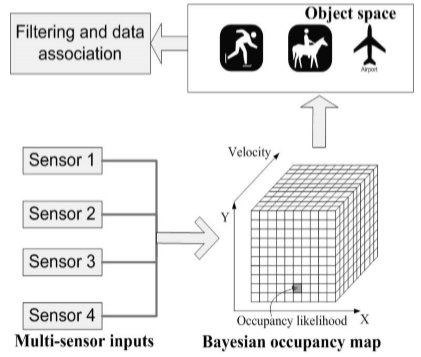
\includegraphics[width=0.9\textwidth]{figs/2-3/bayesian.png}
	\label{fig: object tracking system}
	\caption{基于贝叶斯的占据网格框架。}
\end{figure}

Schindler和Dellaert等人\cite{Schindler2010Probabilistic}利用自下而上的启发式方法,将从SfM管道中的点观测分组为建筑假设和概率时间模型来推断建筑物存在的时间间隔,建立了一个“4D城市”模型。

\begin{figure}[htbp]
	\centering
	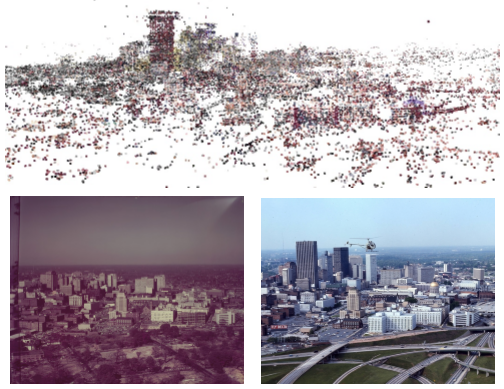
\includegraphics[width=0.9\textwidth]{figs/2-3/city.png}
	\label{fig: 4D city}
	\caption{“4D城市”示意图(1956年-1971年)。}
\end{figure}

Yang和Wang\cite{Yang2011Feasibility}建议用一个“可能性”网格来同时表示静态区域和动态区域。一对对偶传感器模型被用来在移动机器人定位中判别静态及动态物体,然而,他们的工作假定机器人的位置是已知的,具有一定的精度来进行计算以及更新地图,所以该方法并不适合于全局定位问题。

\begin{figure}[htbp]
	\centering
	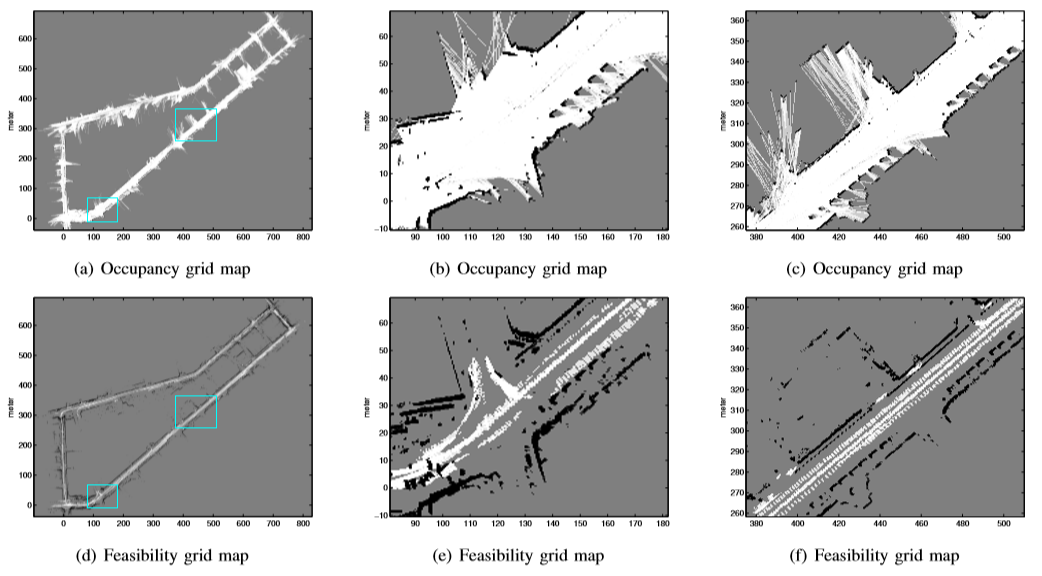
\includegraphics[width=0.9\textwidth]{figs/2-3/feasible.png}
	\label{fig: Grid maps}
	\caption{含“可能性”的网格图。}
\end{figure}

之后,Saarinen\cite{Saarinen2012Independent}等人提出用一系列独立的马尔科夫链去建模整个环境,将状态之间的转换参数建模为两个泊松过程并在线学习这些参数,采用基于近因加权的方法处理非平稳单元的动力学问题。而同样的,该方法也无法普适地应对真实环境下的不同的动态场景及物体。

Murphy\cite{Murphy1999Bayesian}等人建议应用Rao-Blackwellized粒子滤波器来解决SLAM问题并理论上展示了其在动态场景下的可行性。但他们的方法假设了状态转换的概率与环境的当前状态独立并且给定了一个先验,且只能在一个小尺度的环境下工作。之后,Avots等人\cite{Avots2002A},Petrovskaya\cite{Petrovskaya2007Probabilistic}等人分别提出对它的改进,前者用Rao-Blackwellized粒子滤波器来估计机器人的姿态和环境中门的状态,他们使用一个参考占用网格来表示环境,而非他们的状态(其中门的位置是已知的);后者与前者相似,但将门的开关状态这一二元模型改为一个参数化模型(门的打开角度)。而Stachniss和Burgard\cite{Stachniss2005Mobile}也使用Rao-Blackwellized粒子滤波器对聚类后的局部网格图确定的一组可能的环境配置来对机器人进行定位,并从该集合中估计环境的配置。Meyer和Delius\cite{Meyer2010Temporary}跟踪那些由环境中使用临时局部地图的离群对象引起的观测结果,然后用上述粒子滤波器来估计机器人的姿势,该滤波器不仅依赖于这些临时地图,也依赖于环境的参考地图,然而,这项工作仍然依赖于全局定位的静态映射,只有在位置跟踪失败时才会创建临时映射。

另外,对于lifelong的动态环境建图,Konolige\cite{Konolige2009Towards}提出了一个有趣的方法,该方法主要侧重于可视化地图,并提供了一个框架,在该框架中,可以随着时间的推移更新本地地图(视图),并在环境配置更改时添加/删除新的本地地图。Kretzschmar\cite{Kretzschmar2012Information} 等人也给出了类似的想法,他们利用一种有效的信息论图形修剪策略进行图形压缩。该方法可用于偏倚最近的观察结果,以获得与前者工作的类似的表现。然而,这两种方法主要集中在长期操作中出现的可伸缩性问题上,而不是环境随时间变化的动态方面。从这个想法出发,Walcott-Bryant\cite{Walcott2012Dynamic}等人提出了一个名为Dynamic Pose Graph (DPG)的局部表示来建模长时下低动态环境的SLAM问题。

Churchill和Newman\cite{Churchill2012Practice}提出了关于lifelong建图的另一个视角。他们认为导航不需要一个全局参考框架,并介绍了“经验”的概念,即具有相对测量信息的机器人路径。“经验”可以通过基于外观的数据关联方法连接在一起,随着时间的推移而变化的地方由一组不同的“经验”表示。
Tipaldi等人\cite{Tipaldi2013Lifelong}改进并综合了上述基于粒子滤波的方法,提出了一种新的适应环境变化的lifelong 定位方法,它明确地考虑了环境的动态变化,且能够区分表现出高动态行为的物体,例如汽车和人,可以移动并改变配置的物体,例如箱子、架子或门,以及静止不移动的物体,例如墙壁。该方法在二维网格上用一个隐马尔科夫模型描述空间的占据和它的动态性,并通过EM算法学习其参数,联合估计机器人姿态以及全局定位中的环境状态,然后应用一个Rao-Blackwellized粒子滤波器(其中机器人姿态为被采样部分滤波器,网格占据状态为分解的解析部分),同时通过考虑相关马尔可夫链的混合时间来建立一种基于局部地图表示的地图管理方法以能够最小化内存需求,并以合理的概率方式来忘记变化。

\begin{figure}[htbp]
	\centering
	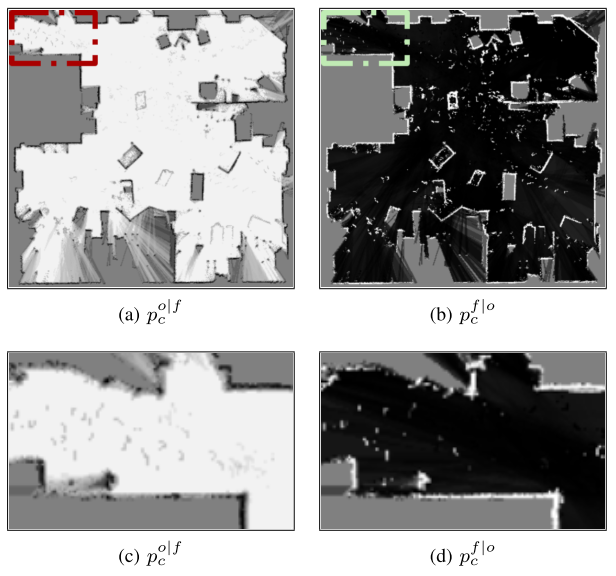
\includegraphics[width=0.9\textwidth]{figs/2-3/filter.png}
	\label{fig:State transition probabilities}
	\caption{状态转移概率示意(颜色越深,概率越大)。}
\end{figure}

之后,Krajník等人\cite{Krajn2014Spectral}提出在光谱域中表示环境动力学,并将其用去图像特征以改进定位,之后也陆续有研究者将该方法应用于占用网格以减少内存需求、应用于拓扑图以改进路径规划。

虽然上述方法适用于移动机器人中使用的大多数环境模型,但由于其依赖于传统的快速傅立叶变换(FFT)方法,因此存在一个主要缺陷,即需要对环境进行定期和定期的观测。这意味着机器人的活动必须分为一个学习阶段,当它经常访问各个位置建立其动态环境模型时,以及当它使用其模型执行有用任务时的部署阶段。这一划分意味着,虽然机器人可以创建更适合长期操作的动态模型,但它不能维护这些模型。因此,机器人不适应那些不存在学习阶段的动力学问题,这会导致其效率随着时间的推移而降低。Krajník等人\cite{Krajnik2015Life}又提出了一种lifelong移动机器人时空动态环境探测的新思路,该方法假设世界处于不断变化的状态,这将为探索空间增加一个额外的时间维度,使探索任务成为一个永无止境的数据收集过程。为了创建和维护一个动态环境的时空模型,机器人不仅要确定在哪里,还要确定何时进行观察。我们将信息论探索应用于世界表征,将环境状态的不确定性建模为时间的概率函数,从而解决这一问题。

\begin{figure}[htbp]
	\centering
	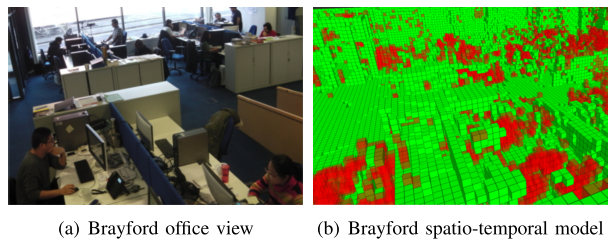
\includegraphics[width=0.9\textwidth]{figs/2-3/lifelong.png}
	\label{fig:Spatio-temporal occupancy grid}
	\caption{随时间变化的占据网格(红色部分)。}
\end{figure}

另外,Ambrus等人\cite{Ambrus2014Meta}提出了一种新的方法来重新创建杂乱的办公环境的静态结构,他们将其定义为“meta-room”,它基于一个配备了rgb-d 深度摄像头的自主机器人在长时间内收集到的多个观测结果进行实验。该方法通过识别从一个观测点到下一个观测点的变化,移除动态元素,同时添加先前被遮挡的对象,以尽可能准确地重建底层静态结构,直接与点簇一起工作。构建meta-room的过程是迭代的,它被设计为在可用时合并新数据,并对环境变化具有鲁棒性。meta-room的最新估计用于区分和提取动态物体群与观测结果。该方法之后也被应用在一些导航机器人平台来得到更好,更细节的物体模型。

\begin{figure}[htbp]
	\centering
	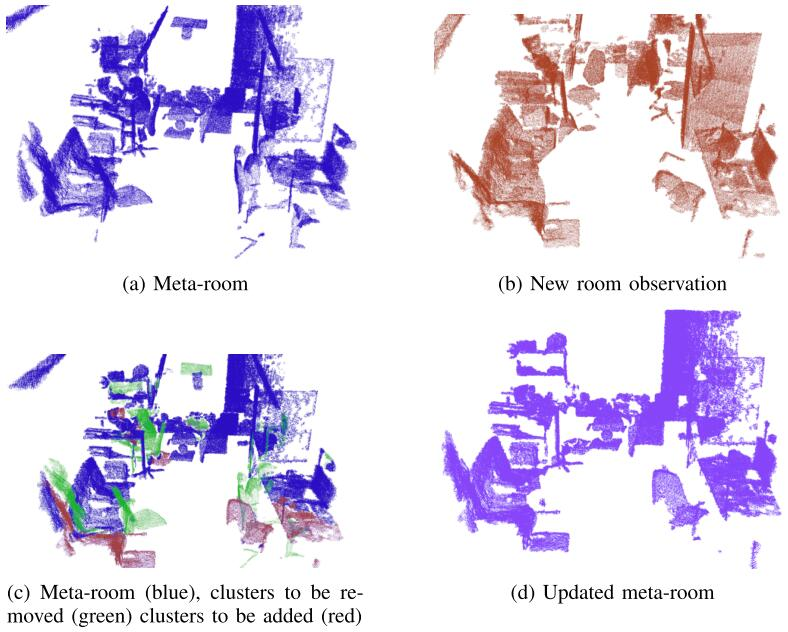
\includegraphics[width=0.9\textwidth]{figs/2-3/meta-room.jpg}
	\label{fig:Meta-room-updating}
	\caption{meta-room更新过程示意。}
\end{figure}

上面提到的Krajnik和Ambrus的工作重点都是使用变化检测算法的结果来分析变化的时空行为,而有的研究人员只关注观测结果之间的变化。Fehr等人\cite{Fehr2017TSDF}提出了一种新的基于扩展截断有符号距离函数(TSDF)的动态场景下的三维重建算法,该算法能够在场景中同时获得动态对象的三维重建的同时,对静态地图进行连续的细化。这是一个具有挑战性的问题,因为地图更新是递增的,并且常常是不完整的。以前的工作通常在点云、曲面或地图上执行变化检测,这些点云、曲面或地图无法区分未探测空间和空白空间。相比之下,该方法基于TSDF的表示自然包含了这些信息,从而使其能够更有力地解决场景差异问题。

\begin{figure}[htbp]
	\centering
	\includegraphics[width=0.9\textwidth]{figs/2-3/TSDF.jpg}
	\label{fig:Change-Detection-Overview}
	\caption{基于TSDF的变化检测框架。}
\end{figure}

总而言之,关于如何将静态和动态场景置于一个统一优美的空间表示形式下,早期研究人员在基于滤波的框架下作了很多的探索,而在面对实际问题时,大部分在真实场景下拥有鲁棒效果的方法却仍然需要沿着前面几个章节所述的技术路线进行。





